\documentclass[a4paper]{scrbook}

\usepackage{fullpage}
\usepackage{style}
\usepackage{tikz-cd}

\newif\iffigureon
\figureonfalse


% THEOREM ENVIORMMENT e.g. \newtheorem{comando}{nome}[numerazione]
\theoremstyle{definition}
\newtheorem{definition}{Definizione}[chapter]
\newtheorem{example}[definition]{Esempio}
\newtheorem{exercise}[definition]{Esercizio}

\theoremstyle{remark}
\newtheorem{oss}[definition]{Osservazione}

\theoremstyle{plain}
\newtheorem{thm}[definition]{Teorema}
\newtheorem{proposition}[definition]{Proposizione}

\newenvironment{solution}{\renewcommand\qedsymbol{}\begin{proof}[Soluzione]}{\end{proof}}

\numberwithin{equation}{chapter}

\title{Introduzione ai sistemi dinamici I}
\author{SciSNS-2017}

\begin{document}

\frontmatter

\maketitle

Quest'opera è stata rilasciata con licenza Creative Commons Attribuzione - Non commerciale - Condividi allo stesso modo 4.0 Internazionale. Per leggere una copia della licenza visita il sito web \url{http://creativecommons.org/licenses/by-nc-sa/4.0/}.
\iffigureon
\begin{center}
  \href{http://creativecommons.org/licenses/by-nc-sa/4.0/}{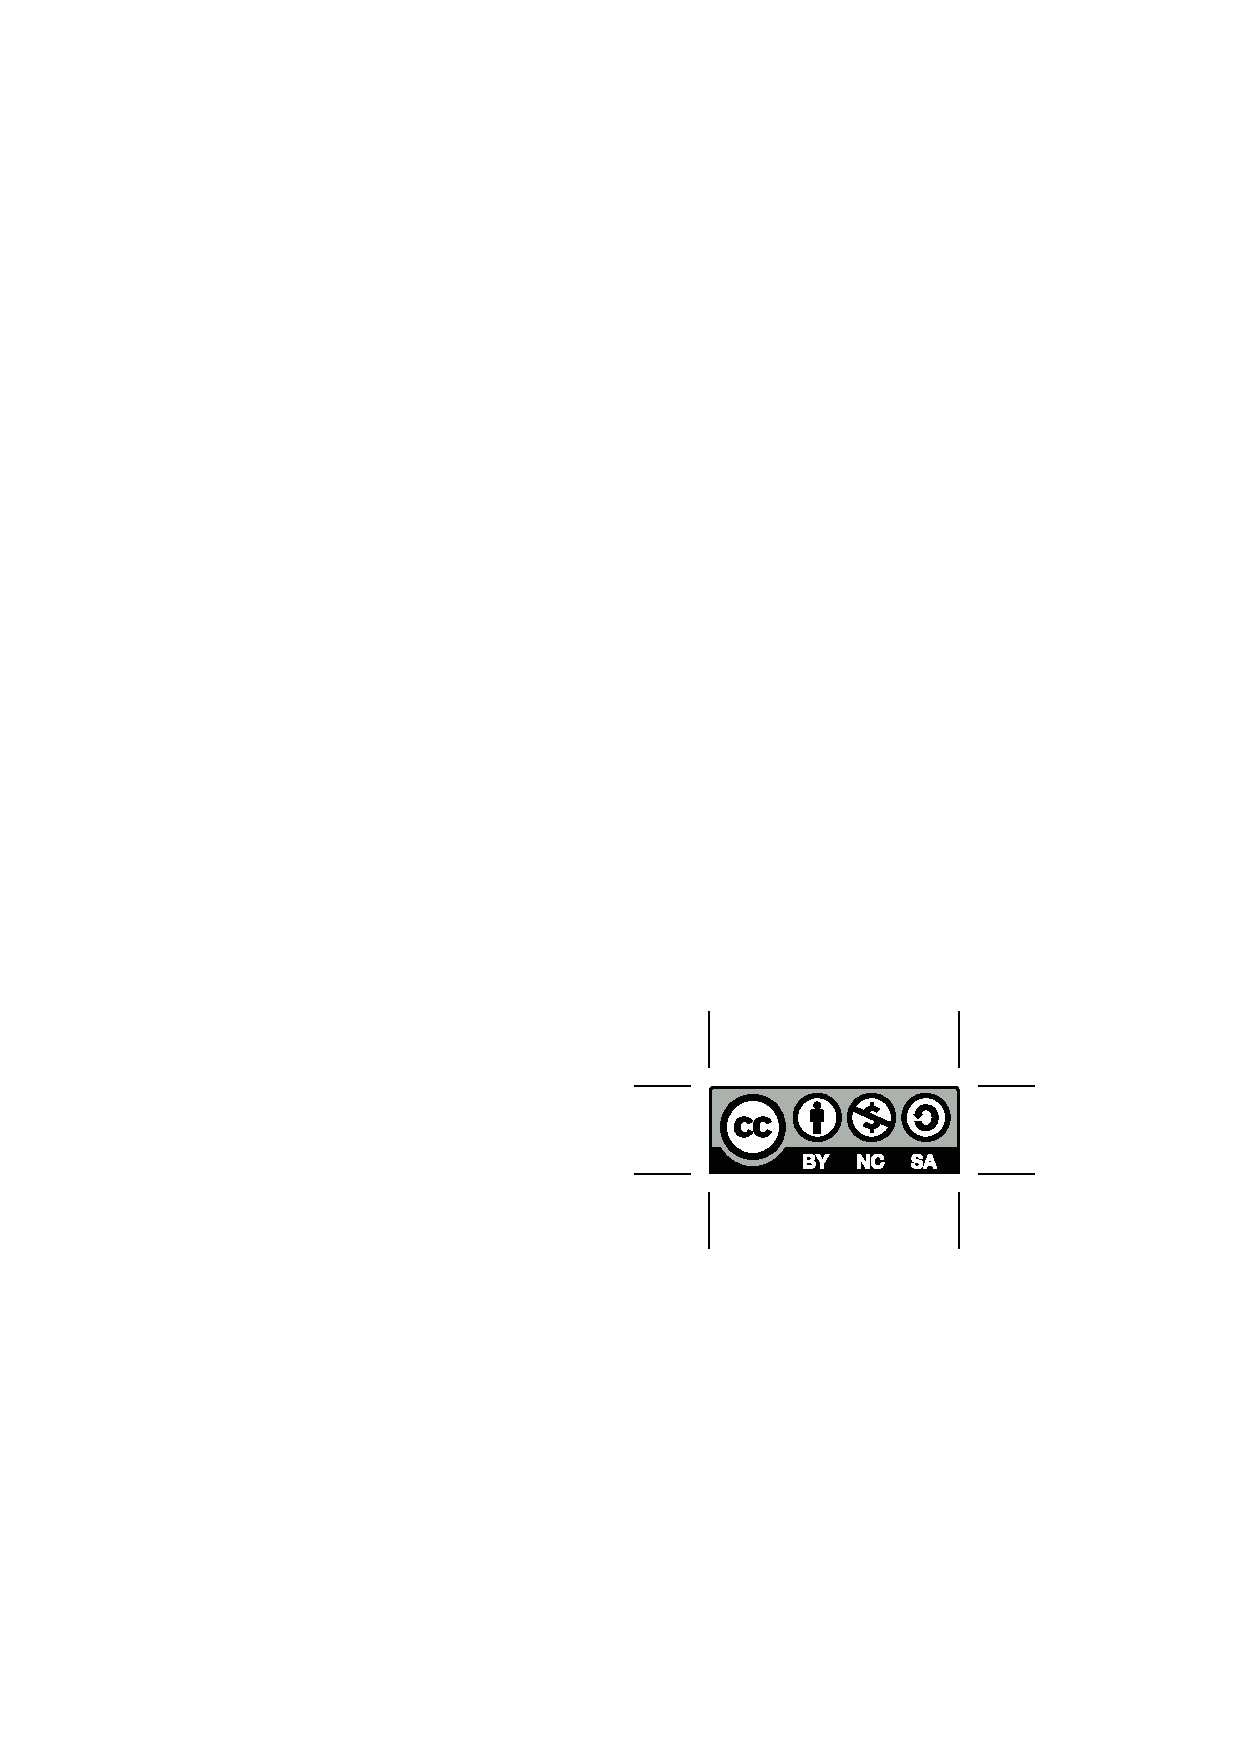
\includegraphics[scale = 0.8]{img/by-nc-sa}}
\end{center}
\fi


\tableofcontents


\mainmatter

\chapter{Lezioni}
\section{Lezione del 09/10/2018}
\begin{definition}[gruppo]
	Un gruppo è una coppia $ \mathcal{G} \coloneqq (G, \star) $ dove $ G $ è un insieme e $ + \colon G \times G \to G $ è un'operazione binaria che gode delle seguenti proprietà
	\begin{enumerate}[label=(\roman*)]
		\item \emph{associativa}: $ \forall g_1, g_2, g_3 \in G, \ g_1 \star (g_2 \star g_3) = (g_1 \star g_2) \star g_3 $;
		\item \emph{elemento neutro sinistro}: $  \exists e \in G : \forall g \in G, \ g \star e = g $;
		\item \emph{inverso sinistro}: $ \forall g \in G, \exists g^{-1} \in G : g \star g^{-1} = e $.
	\end{enumerate}
	A partire da queste si mostra facilmente che l'elemento neutro destro è anche elemento neutro sinistro, l'inverso destro è anche inverso sinistro, che l'elemento neutro e l'inverso sono unici. \\
	Se non ci sono ambiguità circa l'operazione definita su $ G $ indicheremo più semplicemente il gruppo $ \mathcal{G} $ facendo riferimento al solo insieme $ G $. 
\end{definition}

\begin{definition}[sistema dinamico]
	Un sistema dinamico è una terna $ (\mathcal{G}, \mathcal{X}, \Phi) $ dove $ \mathcal{G} \coloneqq (G, \star) $ è un (semi-)gruppo, $ \mathcal{X} $ è uno spazio, cioè un insieme $ X $ dotato di una qualche struttura (per esempio una topologia), e 
	\begin{align*}
		\Phi \colon G \times X & \to X \\
		(g, x) & \mapsto \Phi(g, x) = \Phi_g(x)
	\end{align*}
	è una applicazione tale che
	\begin{enumerate}[label=(\roman*)]
		\item $ \forall x \in X, \ \Phi_e(x) = x $ dove $ e $ è l'elemento neutro di $ G $, cioè $ \Phi_e = \Id_X $;
		\item $ \forall g_1, g_2 \in G, \forall x \in X, \ \Phi_{(g_1 \star g_2)}(x) = (\Phi_{g1} \circ \Phi_{g_2})(x) $ cioè $ \Phi_{(g_1 \star g_2)} = \Phi_{g1} \circ \Phi_{g_2} $.
	\end{enumerate}
	Più brevemente diciamo che un sistema dinamico è l'\emph{azione} di un gruppo $ G $ su uno spazio $ X $ definita da una mappa $ \Phi $. 
\end{definition}

Nella maggior parte dei casi useremo come gruppo insiemi numerici $ \N $, $ \Z $ e $ \R $ con le usuali operazioni. Nei primi due casi parleremo di sistemi a \emph{tempo discreto} mentre nell'ultimo di sistemi a \emph{tempo continuo}. Come spazio $ \mathcal{X} $ useremo spesso uno \emph{spazio metrico compatto} (e.g. la sfera $ \S^d $, il toro $ \T^d $ o un intervallo chiuso $ [a, b] $), uno \emph{spazio di probabilità} o gli insiemi $ \R^d $ e $ \C $ con le usuali strutture. \\

Per quanto riguarda la mappa $ \Phi $ osserviamo che per definizione $ \Phi_g \in \End{(X)} $ ovvero è un \emph{endomorfismo} su $ X $. Tuttavia spesso penseremo a $ \Phi_g \in \Aut{(X)} $ ovvero un \emph{automorfismo} cioè un endomorfismo invertibile. \\

Sia $ f \in \End{(X)} $. Dato $ n \in \N $ poniamo $ f^n \coloneqq f \circ \cdots \circ f $ ($ f $ composta $ n $ volte) con la convenzione che $ f^1 = f $ e $ f^0 = \Id_X $. Se consideriamo $ \N $ con l'operazione di addizione, l'applicazione $ \Phi^f $ data da $ \Phi_n^f(x) \coloneqq f^n(x) $ definisce un sistema dinamico. \\
Se prendiamo $ f \in \Aut{(X)} $ possiamo considerare la stessa costruzione usando come gruppo $ \Z $ e definendo $ f^{-n} $ come l'inversa di $ f^n $. 

\begin{example}
	Partendo dalla costruzione appena data possiamo prendere $ X = [0, 1] $ e per $ \alpha \in \R $ la funzione $ f(x) \coloneqq x + \alpha \pmod{1} $. Osserviamo che essendo $ f $ invertibile possiamo definire l'applicazione $ \Phi $ su $ \Z $. Il sistema così definito è un prototipo di \emph{sistema periodico} se $ \alpha \in \Q $ e di \emph{sistema quasi-periodico} se $ \alpha \notin \Q $. \\
	\texttt{Sarebbe carino mettere un'immagine.}
\end{example}

Prendiamo come gruppo $ \R $ o $ [0, +\infty) $. In tale caso data l'applicazione $ \Phi_t(x) = \Phi(t, x) $ prende il nome di \emph{flusso} o \emph{semi-flusso} rispettivamente. \\

Un esempio di sistema dinamico a tempo continuo è dato da un'equazione differenziale ordinaria (ODE) del primo ordine \footnote{Di seguito considereremo quasi solo ODE del primo ordine in quanto equazioni differenziali di ordine superiore possono essere ricondotte a questa con il solito cambio di variabile a sistemi di ODE del primo ordine.} autonoma
\begin{equation}
	\begin{cases}
		\dot{x} = v(x) \\
		x(0) = x_0
	\end{cases}
\end{equation} 
dove $ x, x_0 \in \R^n $ e $ v \colon \R^n \to \R^n $ è un campo vettoriale. Se supponiamo che $ v $ sia di classe $ \mathcal{C}^1 $ allora abbiamo esistenza e unicità della soluzione \texttt{(e dipendenza continua dai parametri iniziali ??)}, cioè esiste $ \tau > 0 $ e un'unica funzione $ \phi \colon [0, \tau) \to \R^n $ tale che $ \phi(0) = x_0 $ e $ \phi'(t) = v(\phi(0)) $ per ogni $ t \in [0, \tau) $. \\
Se supponiamo per esempio che $ v $ sia un'applicazione lineare $ v(x) \coloneqq A x $ con $ A \in \mathrm{Mat}_{n \times n}(\R) $ allora abbiamo che la soluzione è prolungabile a tutto l'asse reale e introducendo la nozione di esponenziale di una matrice %
\footnote{%
	Data $ A \in \mathrm{Mat}_{n \times n}(\R) $ si pone 
	\[
		\exp(A) \coloneqq \sum_{k = 0}^{+\infty} \frac{A^k}{k!}.
	\] 
} si può scrivere nella forma 
\[
	\phi(t) = \exp{\left(t \, A\right)} \, x_0. 
\]


\begin{definition}[orbita e spazio delle orbite]
	Data $ f \in \Aut{(X)} $ e $ \Phi^f \colon \Z \times X \to X $ definiamo orbita di $ x \in X $ come 
	\[
	\mathcal{O}^f(x) \coloneqq \{f^n(x) : n \in \Z\}.
	\]
	Le orbite definiscono una naturale relazione di equivalenza $ x \sim y \iff \exists n \in \Z : y = f^n(x) \iff y \in \mathcal{O}^f(x) \iff x \in \mathcal{O}^f(y) $. Chiamiamo lo spazio quoziente $ \faktor{X}{\sim} $ spazio delle orbite. \texttt{Topologia quoziente?}
\end{definition}

Pendolo semplice...

\section{Lezione del 10/10/2018}
\subsection{Introduzione}
La Teoria della Misura nasce a inizio '900 per formalizzare la probabilità e per cercare di fondare una teoria dell'integrazione che risulti più efficace di quella di Riemann. Per alcuni sottoinsiemi di $\R$, in particolare per gli intervalli limitati, abbiamo un concetto intuitivo di "misura", ovvero la lunghezza dell'intervallo:
\[\lambda\left([a,b]\right) = b-a.\]
L'obiettivo della teoria della misura è estendere questa nozione ad altri sottoinsiemi di $\R$ in modo coerente, ovvero in modo da rispettare, ad esempio, la proprietà di additività:
\[A \cap B = \emptyset \implies \lambda(A\cup B) = \lambda(A) + \lambda(B)\]
\section{Lezione del 17/10/2018 [Grotto]}
\subsection{Integrali}
\begin{definition}[Integrale di una funzione semplice]
    Sia $ (X,\mathcal{F},\mu) $ uno spazio di misura e sia $ \phi\colon X\to [0,+\infty] $ una funzione semplice $ \phi(x) \coloneqq \sum_{i=1}^N a_i\chi_{A_i}(x)$ con $ a_i\in[0,+\infty] $. Definiamo l'integrale di $ \phi $ come:
    \[ \int_X \phi(x)\dif\mu(x) \coloneqq \sum_{i=1}^{N} a_i \mu(A_i) \]
\end{definition}
\begin{definition}[Integrale di funzioni non negative]
    Sia $ f\colon X\to [0,+\infty] $ una funzione misurabile. Definiamo il suo integrale come:
    \[ \int_X f(x)\dif\mu(x) \coloneqq \sup\left\{ \int_X \phi(x)\dif\mu(x) : 0 \leq \phi(x) \leq f(x) \text{ con $\phi$ semplice} \right\} \]
    Se l'integrale di $ f $ è finito, questa si dirà \emph{integrabile} o \emph{sommabile}.
\end{definition}
\begin{definition}[Integrale]
    Data $ f\colon X\to\R $ e dette $ f^+(x) = \max\left\{f(x),0\right\} $ e $ f^-(x) = \max\left\{-f(x), 0\right\} $, $ f $ si dice \emph{integrabile} o \emph{sommabile} se lo sono $ f^+ $ e $ f^- $ e in tal caso si pone:
    \[ \int_X f(x)\dif\mu(x) \coloneqq \int_X f^+(x)\dif\mu(x) - \int_X f^-(x)\dif\mu(x) \]
    Se infine $ f\colon X\to\C $ si pone:
    \[ \int_X f(x)\dif\mu(x) \coloneqq \int_X\Re[f(x)]\dif\mu(x) + i\int_X\Im[f(x)]\dif\mu(x) \]
\end{definition}
Elenchiamo alcune proprietà dell'integrale di una funzione $ f\colon X\to \R $:
\begin{enumerate}
    \item \emph{Monotonia}: $ 0 \leq g \leq f \Rightarrow \int\! g\dif\mu \leq \int\! f\dif\mu $;
    \item \label{it:quasi_ovunque}Se $ f=g $ quasi ovunque, allora $ \int f\dif\mu = \int g\dif\mu $;
    \item Sia $ \mu $ una misura su $ X $ e $ \bar{\mu} $ il suo completamento. Allora $ \int_X f\dif\mu = \int_X f\dif\bar{\mu} $;
    \item L'integrale è lineare rispetto all'integranda;
    \item $ f $ è misurabile se e solo se $ \abs{f} $ è integrabile e in tal caso vale:
    \[ \abs{ \int_X f(x)\dif\mu(x)} \leq \int_X \abs{f(x)}\dif\mu(x) \]
    \item I seguenti fatti sono equivalenti:
    \begin{enumerate}[label=(\roman*)]
        \item $ \int_X \abs{f(x)}\dif\mu(x) = 0$;
        \item $ f = 0 $ quasi ovunque;
        \item $ \int_A f(x)\dif\mu(x) $ \textcolor{red}{Boh...} $ \forall A\in\mathcal{F} $ \footnote{Si pone $ \int_A f(x)\dif\mu(x) \coloneqq \int_A f\rvert_A(x) \dif\mu\rvert_A(x) $}.
    \end{enumerate}
\end{enumerate}
\begin{definition}
    Chiamiamo $ \mathscr{L}^1(X,\mathcal{F},\mu) $ lo spazio delle funzioni (misurabili) integrabili.
\end{definition}
\begin{exercise}[Disuguaglianza di Markov]
    Sia $ f\in\mathscr{L}^1(X,\mathcal{F},\mu) $ con $ f\geq 0 $ e sia $ \lambda > 0 $. Allora:
    \[ \mu\left( \left\{ x\in X : f(x) \ge \lambda \right\}  \right) \leq \frac{1}{\lambda}\int_X f(x)\dif\mu(x) \]
\end{exercise}
\begin{proof}
    $ \lambda\mu\left( \{ f \geq \lambda \} \right) = \int_X \chi_{ \{f\geq\lambda \} } \lambda \dif\mu = \int_{ \{ f \geq \lambda \} } \lambda \dif\mu \leq \int_{ \{ f \geq \lambda \} } f\dif\mu \leq \int_X f\dif\mu $
\end{proof}
\begin{thm}[Beppo Levi o Convergenza Monotona]
    Sia $ (f_n)_{n\in\N} $ una successione di funzioni misurabili con $ f_n \geq 0 $ e sia $ f\colon X\to[0,+\infty] $ tale che $ f_n\nearrow f $ quasi ovunque. Allora $ f $ è misurabile e vale:
    \[ \int_X f(x)\dif\mu(x) = \lim_{n\to+\infty} \int_X f_n(x)\dif\mu(x) \]
\end{thm}
\begin{proof}
    \textcolor{red}{content}
\end{proof}
\begin{exercise}[Assoluta continuità]
    Dimostrare che per ogni $ f \in \mathscr{L}^1(X,\mathcal{F},\mu) $ vale:
    \[ \quad \forall\epsilon > 0\ \exists \delta > 0 : \forall A\in\mathcal{F}\ \mu(A) < \delta \Rightarrow \int_A \abs{f(x)} \dif\mu(x) < \epsilon \]
\end{exercise}
\begin{exercise}[Lemma di Fatou]
    Siano $ (f_n) $ con $ f_n\colon X\to[0,+\infty] $ misurabili. Allora:
    \[ \int_X \liminf_{n\to +\infty}f_n(x)\dif\mu(x) \leq \liminf_{n\to +\infty} \int_X f_n(x)\dif\mu(x) \]
\end{exercise}
\begin{exercise}[Convergenza dominata]
    Siano $ f, f_n\colon X\to\R $ tali che $ f_n\to f $ quasi ovunque. Sia $ g\in\mathscr{L}^1(X) $ con:
    \[ \abs{f_n(x)} \leq g(x) \text{ quasi ovunque} \]
    Allora $ f $ è integrabile e vale:
    \[ \int_X f(x)\dif\mu(x) = \lim_{n\to +\infty}\int_X f_n(x)\dif\mu(x) \]
\end{exercise}
\begin{exercise}[Disuguaglianza di Jensen]
    Sia $ \mu $ una misura di probabilità su $ X $, $ f\in\mathscr{L}^1(X) $, $ \phi\colon \R\to\R $ convessa. Allora:
    \[ \phi\left(\int_X f(x)\dif\mu(x) \right) \leq \int_X (\phi\circ f)(x)\dif\mu(x) \]
\end{exercise}
\subsection{Spazi $ L^p $}
\begin{definition}[Spazi $ \mathscr{L}^p $]
    Sia $ (X,\mathcal{F},\mu) $ uno spazio di misura e $ p\in[0,+\infty) $. Definiamo:
    \[ \mathscr{L}^p(X,\mathcal{F},\mu) \coloneqq \left\{ f\colon X\to \R : \int_X \abs{f(x)}^p \dif\mu(x) < +\infty \right\}  \]
    Su tale spazio definiamo una \emph{semi-norma}:\footnote{Ossia una ``norma'' per cui non vale $ \norm{v} = 0 \Rightarrow v=0 $.}
    \[ \norm{f}_p \coloneqq \left( \int_X \abs{f(x)}^p\dif\mu(x) \right)^{\frac{1}{p}} \]
\end{definition}
\begin{exercise}[Disuguaglianza di Hölder]
    Siano $ p, q \in [1,+\infty) $ con $ \frac{1}{p} + \frac{1}{q} = 1 $. Allora $ \forall f,g \in \mathscr{L}^1 $ vale:
    \[ \norm{fg}_{1} \leq \norm{f}_p\norm{g}_q \]
\end{exercise}
\begin{exercise}[Disuguaglianza di Minkowski]
    Sia $ p\in[1,+\infty) $ e siano $ f,g \in\mathscr{L}^p$. Allora $ f+g \in\mathscr{L}^p $ e vale:
    \[ \norm{f+g}_p \leq \norm{f}_p + \norm{g}_p \]
\end{exercise}

Al fine di ottenere un vero spazio normato, quozientiamo $ \mathscr{L}^p $ per un'opportuna relazione di equivalenza, definita come:
\[ f \sim g \iff f = g \text{ quasi ovunque} \]
Abbiamo dunque:
\[ L^p(X,\mathcal{F},\mu) \coloneqq \faktor{\mathscr{L}^p(X,\mathcal{F},\mu)}{\sim} \]
La \emph{quasi-norma} passa al quoziente per la proprietà \eqref{it:quasi_ovunque} e diventa una vera norma.

Notiamo che gli elementi di $ L^p $ sono \emph{classi di equivalenza} di funzioni, ma d'ora in poi, per semplicità, diremo che sono semplicemente \emph{funzioni}, sottintendendo che si sta scegliendo un rappresentante della classe di equivalenza in questione.

\subsection{Misure prodotto e integrali multipli}
Siano $ (X,\mathcal{E},\mu) $ e $ (Y,\mathcal{F},\nu) $ spazi di misura $ \sigma $-finiti. Definiamo:
\[ \mathcal{E} \otimes \mathcal{F} \coloneqq \left\{ E\times F : E \in \mathcal{E}, F \in \mathcal{F} \right\} \]
Dato $ A \in \mathcal{E}\otimes\mathcal{F} $, $ \pi_x(A) $ e $ \pi_y(A) $ (\textcolor{red}{sezioni di A a $ x $ o $ y $ fissate}) sono $ \mathcal{F} $- e $ \mathcal{E} $-misurabili rispettivamente.
Esiste unica una misura $ \mu\otimes\nu $ su $ (X\times Y, \mathcal{E}\otimes\mathcal{F}) $ che estende
\[ (\mu\otimes\nu)(E\times F) = \mu(E)\mu(F) \qquad \forall E\in\mathcal{E}\ \forall F\in\mathcal{F} \]
\[ (\mu\otimes\nu)(A) = \int_X \nu(\pi_x A)\dif\mu(x) = \int_Y \mu(\pi_y A)\dif\nu(y) \]
\begin{thm}[Tonelli]\label{thm:Tonelli}
    Sia $ f\colon X\times Y \to [0,+\infty] $ misurabile su $ (X\times Y,\mathcal{E}\otimes\mathcal{F}) $. Allora:
    \[ \int_{X\times Y} f(x,y)\dif(\mu\otimes\nu)(x,y) = \int_X \left( \int_Y f(x,y) \dif\nu(y) \right) \dif\mu(x) = \int_Y \left( \int_X f(x,y) \dif\mu(x) \right) \dif\nu(y) \]
\end{thm}
\begin{thm}[Fubini]
    Sia $ f \in L^1(X\times Y,\mathcal{E}\otimes\mathcal{Y},\mu\otimes\nu) $. Allora vale la tesi del teorema \ref{thm:Tonelli} per funzioni a valori di segno qualsiasi.
\end{thm}

\subsection{Cambi di variabili}
Dato $ (X,\mathcal{F},\mu) $ $ \sigma $-finito, $ f\colon X\to[0,+\infty] $ misurabile, chiamiamo \emph{misura con densità} una del tipo:
\[ \nu(A) \coloneqq \int_A f(x)\dif\mu(x) \]
Se $ f $ è anche integrabile, allora la misura con densità è una misura finita.
\begin{example}[Gaussiana su $ \R $]
    \[ \dif\mu(x) = \frac{1}{\sqrt{2\pi\sigma^2}} \exp{\left (-\frac{x^2}{2\sigma}\right )} \dif x \]
\end{example}
\begin{example}[Distribuzione di Cauchy]
    \[ \dif\mu(x) = \frac{1}{\pi(1+x^2)}\dif x \]
\end{example}

\begin{definition}[Assoluta continuità delle misure]
    Date due misure $ \mu $ e $ \nu $ diciamo che $ \nu $ è \emph{assolutamente continua} rispetto a $ \mu $ ($ \nu \ll \mu $) se vale $ \mu(A) = 0 \Rightarrow \nu(A) = 0\ \forall A $
\end{definition}
\begin{thm}[Radon-Nicodym]
    Se $ \nu \ll \mu $, allora $ \exists f\colon X\to [0,+\infty] $ misurabile tale che $ \nu(A) = \int_A f(x)\dif\mu(x) $.
\end{thm}

\begin{thm}[Cambio di variabile per funzioni lisce]
    Sia $ V \subseteq\R^d $ aperto, $ W\subseteq\R^d $ aperto limitato e $ T\colon V\subseteq \R^d \to W \subseteq \R^d $ differenziabile, invertibile con inversa continua. Allora $ \forall f\in L^1(W) $
    \[ \int_W f(y)\dif y = \int_V f(T(x)) \abs{\det{\jac{T}(x)}} \dif x \]
\end{thm}
\begin{oss}
    Data $ \dif\mu(x) = \rho(x)\dif x $, $ \dif(T_\sharp\mu)(y) = \rho(T^{-1}(y)) \abs{\det{\jac T}(T^{-1}(y))}^{-1} \dif y $.
\end{oss}

\textcolor{red}{Cose su misure invarianti.}

\begin{exercise}[Mappa logistica]
    Sia $ Q\colon [0,1] \to [0,1] $ definita come $ Q(x) = 4x(1-x) $; una misura invariante è:
    \[ \dif\mu(x) = \frac{\dif x}{\pi\sqrt{x(1-x)}} \]
\end{exercise}
\begin{exercise}
    Sia $ N\colon \R\to\R $ definita come $ N(x) = \frac{1}{2} \left( x-\frac{1}{x} \right) $; una misura invariante è:
    \[ \dif y(x) = \frac{\dif x}{\pi(1+x^2)} \]
\end{exercise}

\section{Lezione del 24/10/2018 [Marmi]}

\begin{definition}[numero algebrico]
	Un numero $ \alpha $ in $ \R $ o $ \C $ si dice algebrico se è radice di un polinomio a coefficienti interi, cioè se esiste $ P \in \Z[x] $ tale che $ P(\alpha) = 0 $. \\
	Si definisce \emph{grado} $ d $ di $ \alpha $ se $ \alpha $ è radice di un polinomio di grado $ d $ e di nessun polinomio di grado minore.  
\end{definition}

\begin{thm}[Liouville]
	Se $ \alpha $ è algebrico di grado $ d \geq 2 $ allora $ \forall \epsilon > 0 $ la disequazione
	\[
		\abs{\alpha - \frac{p}{q}} < \frac{1}{q^{d + \epsilon}}
	\]
	ha solo un numero finito di soluzioni. 
\end{thm}
%
\begin{proof}
	Sia $ P \in \Z[x] $ di grado $ d $ indivisibile tale che $ P(\alpha) = 0 $. Osserviamo che per ogni $ p/q \in \Q $ diverso da $ \alpha $ vale che $ P(p/q) = N/q^d $ per un qualche $ N \in \Z \setminus \{0\} $. \\
	Lo sviluppo in serie di Taylor di $ P $ centrato in $ \alpha $ ha espressione finita e pari a 
	\[
		P(x) = \sum_{k = 1}^{d} \frac{P^{(k)}(\alpha)}{k!} (x - \alpha)^k
	\]
	dove abbiamo omesso il termine di grado zero essendo $ P^{(0)}(\alpha) = P(\alpha) = 0 $. Così
	\[
		\abs{P\left(\frac{p}{q}\right)} \leq \sum_{k = 1}^{d} \frac{\abs{P^{(k)}(\alpha)}}{k!} \abs{\frac{p}{q} - \alpha}^k = \abs{\frac{p}{q} - \alpha} \sum_{k = 1}^{d} \frac{\abs{P^{(k)}(\alpha)}}{k!} \abs{\frac{p}{q} - \alpha}^{k - 1}.
	\]
	Se $ \abs{p/q - \alpha} \leq 1 $, posto $ A(\alpha) \coloneqq d \sup_{1 \leq k \leq d} \frac{1}{k!} \abs{P^{(k)}(\alpha)} $ otteniamo 
	\[
		\frac{\abs{N}}{q^d} \leq \abs{\frac{p}{q} - \alpha} A(\alpha).
	\]
\end{proof}

\subsection{Back to dinamica topologica}
\emph{Setting}: $ (X, d) $ è uno spazio metrico compatto, $ f \colon X \to X $ è una funzione continua e la dinamica è quella data dall'iterazione di $ f $. 

\begin{definition}[funzione topologicamente transitiva]
	$ f $ si dice topologicamente transitiva se esiste un punto la cui orbita è densa cioè $ \exists x \in X : \overline{\mathcal{O}_f(x)} = X $.
\end{definition}

\begin{definition}[funzione minimale]
	$ f $ si dice minimale se $ \forall x \in X, \ \overline{\mathcal{O}_f(x)} = X $. 
\end{definition}

\begin{definition}[insieme minimale]
	Un insieme chiuso, $ f $-invariante e non vuoto $ A \subseteq X $ si dice minimale se $ f\lvert_A $ è minimale. 
\end{definition}

Osserviamo che la transitività topologica così come la minimalità sono invarianti per coniugazione o semi-coniugazione topologica.

\begin{thm}
	Sia $ f \colon X \to X $ un omeomorfismo. I seguenti fatti sono equivalenti.
	\begin{enumerate}[label=(\roman*)]
		\item $ f $ è topologicamente transitiva.
		\item \emph{Idemcomponibilità topologica}: se $ U \subseteq X $ è aperto $ f $-totalmente invariante, i.e. $ U = f(U) = f^{-1}(U) $, allora $ U = \emptyset $ o $ \overline{U} = X $.
		\item Per ogni coppia di aperti non vuoti $ U, V \subseteq X $ esiste un $ n_0 \in \Z $ tale che $ f^{n_0}(U) \cap V \neq \emptyset $. 
		\item $ \{x \in X : \overline{\mathcal{O}_f(x)} = X\} $ è un $ G_\delta $-denso\footnote{%
			Un sottoinsieme $ A $ di uno spazio topologico $ (X, \tau) $ si dice $ G_\delta $-denso se è intersezione numerabile di aperti densi. 
		}.
	\end{enumerate}
\end{thm}
%
\begin{proof}
	Mostriamo le varie implicazioni. 
	\begin{enumerate}
		\item[$ (i) \Rightarrow (ii) $] Per ipotesi $ \exists x \in X : \overline{\mathcal{O}_f(x)} = X $. Allora se $ U \neq \emptyset, \ \exists n \in \Z : f^{n}(U) \in U $ da cui essendo $ f $-totalmente invariante, $ \forall n \in Z, \ f^n(x) \in U $ ovvero $ \overline{U} = \overline{\mathcal{O}_f(x)} = X $. 
		\item[$ (ii) \Rightarrow (iii) $] Dato $ U $ aperto e non vuoto costruiamo un aperto non vuoto e $ f $-totalmente invariante ponendo $ U' \coloneqq \bigcup_{n \in \Z} f^n(U) $. Per ipotesi $ \overline{U'} = X $ da cui $ U' \cap V \neq \emptyset $. Allora per definizione $ \exists n_0 \in \Z : f^{n_0}(U) \cap V \neq \emptyset $.
		\item[$ (iii) \Rightarrow (iv) $] Ricordiamo che gli spazi metrici compatti sono \emph{spazi polacchi} cioè ammettono una base numerabile di aperti $ \{U_i\}_{i \in \N} $. Osserviamo che il fatto che $ \overline{\mathcal{O}_f(x)} = X $ è equivalente a chiedere che $ \forall n \in \N, \ \exists j \in \Z : f^j(x) \in U_n $ e cioè che $ x \in \bigcap_{n \in \N} \bigcup_{m \in \Z} f^{m}(U_n) $. Ora per ipotesi $ \bigcup_{m \in \Z} f^m(x) $ ha intersezione non vuota con ogni aperto non vuoto, cioè è denso in $ X $. Per definizione questo implica che $ \{x \in X : \overline{\mathcal{O}_f(x)} = X\} $ è un $ G_\delta $-denso. 
		\item[$ (iv) \Rightarrow (i) $] Essendo $ \{x \in X : \overline{\mathcal{O}_f(x)} = X\} $ un $ G_\delta $-denso per il Teorema di Ba\^{i}re è anche un denso e pertanto non vuoto. Dunque $ \exists x \in X : \overline{\mathcal{O}_f(x)} = X $ cioè $ f $ è topologicamente transitiva. \qedhere
	\end{enumerate}
\end{proof}

Osserviamo che se $ f \colon X \to X $ è solo continua allora $ (i) $ e $ (ii) $ sono comunque equivalenti a patto che $ X $ non abbia punti isolati. \\

\begin{definition}[integrale primo]
	Un integrale primo è una funzione $ \varphi \colon X \to \R $ tale che $ \varphi \circ f = \varphi $, cioè che è costante sulle orbite. 
\end{definition}

\begin{proposition}
	Se $ f $ è topologicamente transitiva allora gli unici integrali primi continui sono funzioni costanti.
\end{proposition}
%
\begin{proof}
	Se $ \varphi $ è un integrale primo allora $ \varphi(\mathcal{O}_f(\bar{x})) = c $ con $ c \in \R $ dove $ \bar{x} \in X $ è il punto le cui orbite sono dense in $ X $. Allora se $ x \in \R $ esiste una successione $ (x_k)_{k \in \N} \subseteq \mathcal{O}_f(\bar{x}) $ tale che $ x_k \to x $. Essendo $ \varphi $ continua allora $ \varphi(x) = \lim_{k} \varphi(x_k) = \lim_{k} c = c $ da cui segue la tesi. 
\end{proof}

\begin{definition}[topologicamente mescolante]
	Una dinamica definita da $ f $ si dice topologicamente mescolante se $ \forall U, V $ aperti non vuoti $ \exists n_0 \in \N : \forall n \geq n_0, \ f^n(U) \cap V \neq \emptyset $. 
\end{definition}

\begin{example}[dilatazione sul toro e shift]
	Fissato $ m \geq 2 $ intero sia $ E_m \colon \T^1 \to \T^1 $ data da $ E_m(x) \coloneqq mx \pmod{1} $. Su $ \T^1 $ poniamo la distanza euclidea modulo 1, cioè $ d(x, y) = \inf_{p \in \Z} \abs{x - y - p} $ rispetto alla quale è uno spazio metrico compatto. Osserviamo i seguenti fatti
	\begin{itemize}
		\item $ E_m $ è una mappa \emph{espansiva}, cioè se $ x, y \in \T^1 $ e $ d(x, y) < 1/2^n $ allora $ d(E_m(x), E_m(y)) = m d(x, y) $ per un qualche $ n $. (??)
		\item $ E_m $ conserva la misura di Lebesgue 
		\item $ E_m $ è un fattore dello \emph{shift su $ m $ simboli}. \\
		Posto $ \Sigma_m \coloneqq \{0, 1, \ldots, m-1\}^{\N} $ definiamo la mappa $ \sigma \colon \Sigma_m \to \Sigma_m $ di shift su $ m $ simboli che dato un elemento $ (\epsilon_i)_{i \in \N} \in \Sigma_m $ agisce sulla successione avanzando di uno gli indici $ \sigma\left((\epsilon_i)_{i \in \N}\right) \coloneqq (\epsilon_{i + 1})_{i \in \N} $. \\
		Sull'insieme $ \Sigma_m $ è possibile definire un concetto di \emph{profondità} dalla quale si separano due successioni come 
		\[
			a\left((\epsilon_i), (\delta_i)\right) \coloneqq \inf_{i \in \N} \{\epsilon_i \neq \delta_i\}
		\]
		a partire dalla quale possiamo definire una distanza tra successioni 
		\[
			d\left((\epsilon_i), (\delta_i)\right) \coloneqq m^{-a\left((\epsilon_i), (\delta_i)\right)}. 
		\]
		Rispetto a tale distanza $ \Sigma_m $ è uno spazio metrico compatto e $ \sigma $ è una funzione continua ma non è un omeomorfismo. Ciò è invece vero se al posto di $ \Sigma_m $ si considera l'insieme delle successioni bi-infinite $ \tilde{\Sigma}_m \coloneqq \{0, 1, \ldots, m-1\}^{\Z} $. \\
		Prima di tutto mostriamo che $ d $ è una distanza. La proprietà simmetrica è ovvia per costruzione così come il fatto che $ d $ sia positiva. Se $ d((x_i), (y_i)) = 0 $ allora $ a((x_i), (y_i) = +\infty $ ovvero $ x = y $. Per quanto riguarda la disuguaglianza triangolare dobbiamo mostrare che $ \forall (x_i), (y_i), (z_i) \in \Sigma_m $ si ha $ m^{-a((x_i),(z_i))} \leq m^{-a((x_i), (y_i))} + m^{-a((y_i), (z_i))} $. Siano $ \alpha \coloneqq a((x_i), (z_i)) $ e $ \beta \coloneqq a((x_i)) $. Se $ \alpha = \beta $ allora la disuguaglianza è verificata. Se $ \alpha < \beta $ allora $ \forall i \leq \beta-1, \ x_i = y_i $ ed essendo $ x_\alpha \neq z_\alpha $ otteniamo che $ z_\alpha \neq y_\alpha $ e $ \forall i \leq \alpha-1, \ z_i = y_i $, cioè $ a((y_i), (z_i)) = \alpha $. Viceversa se $ \alpha > \beta $ allora $ \forall i \leq \beta-1, x_i=y_i=z_i $ e inoltre $ x_\beta=z_\beta \neq y_\beta $ quindi $ a((y_i), (z_i)) = \beta $: osservando che $ m, \alpha, \beta \in \N $ e che $ m \geq 2 $ abbiamo che $ \alpha > \beta \Rightarrow \alpha \geq \beta - 1 \geq \beta - \log_m 2 $ per ogni $ m $, da cui otteniamo che $ m^{-\alpha} \leq 2m^{-\beta} $ che è la disuguaglianza voluta. \\
        Per mostrare la compattezza verifichiamo che $ \Sigma_m $ è totalmente limitato e completo.
        \begin{itemize}
            \item Le palle di raggio $ R $ e di centro $ \bar{x} \coloneqq (\bar{x}_i)_{i \in \N} $ di questo spazio metrico sono 
            \[
            B_R(\bar{x}) = \{(x_i) \in \Sigma_m : \forall i \in \N : 0 \leq i \leq -\log_m{R}, \ x_i = \bar{x}_i\}.
            \] 
            Osserviamo quindi che, posto $ p \coloneqq \left \lfloor -\log_m{R} \right \rfloor $, ogni successione della forma \linebreak $ (x_1, \ldots, x_p, x_{p+1}, \ldots) $ stà in $ B_R{\left((x_1, \ldots, x_p, 0, \ldots)\right)} $ e pertanto considerando l'insieme delle possibili $ m^p $ successioni distinte che sono costantemente nulle dal $ p+1 $-esimo termine in poi, le palle di raggio $ R $ centrate in tali elementi sono un ricoprimento finito di $ \Sigma_m $. 
            \item Sia ora $ (x^j)_{j \in \N} \coloneqq ((x_i^j)_{i \in \N})_{j \in \N} $ una successione di Cauchy in $ \Sigma_m $, cioè tale che $ \forall \epsilon > 0, \ \exists \bar{j} : \forall j_1, j_2 \geq \bar{j}, \ x_i^{j_1} = x_i^{j_2} \ \forall i \leq -\log_m{\epsilon} $. Essendo la successione $ (x_i^j)_{j \in \N} $ definitivamente costante (a $ i $ fissato, scelto un $ \epsilon $ positivo tale che $ -\log_m{\epsilon} > i $, per la proprietà di Cauchy abbiamo che $ \exists \bar{j} : \forall j \geq \bar{j}, \ x_i^j = \text{cost} $) possiamo porre $ \bar{x}_i \coloneqq \lim_{j \to +\infty} x_i^j $. La successione $ \bar{x} \coloneqq (\bar{x}_i)_{i \in \N} $ è il candidato limite. Dobbiamo mostrare che $ \lim_{j \to +\infty} d(x^j, \bar{x}) = 0 $, cioè che $ \forall I, \ \exists \bar{j} : \forall j \geq \bar{j}, \ \inf{\{i : x_i^j \neq \bar{x}_i\}} \geq I $. Tale proprietà è verificata per costruzione: fissato $ I \in \N $, per ogni $ i \in \{0, \ldots, I\} $ sappiamo che esiste $ j_i \in \N : \forall j \geq j_i, \ x_i^j = \bar{x}_i $; prendendo allora $ \bar{j} \coloneqq \max \{j_1, \ldots, j_I\} $ otteniamo che per ogni $ 0 \leq i \leq I $ e $ \forall j \geq \bar{j} $ si ha $ x_i^j = \bar{x}_i $, cioè $ \inf{\{i : x_i^j \neq \bar{x}_i\}} \geq I $. 
        \end{itemize} 
	\end{itemize}
\end{example}




%\appendix

%\chapter{Appendice}


%\backmatter

%\bibliography{bibliografia}


\end{document}
